\documentclass[12pt]{article}
\usepackage[utf8]{inputenc}
\usepackage[spanish,es-lcroman, es-tabla]{babel}
\usepackage[autostyle,spanish=mexican]{csquotes}
\usepackage{amsmath}
\usepackage{amssymb}
\usepackage{nccmath}
\numberwithin{equation}{section}
\usepackage{amsthm}
\usepackage{graphicx}
\usepackage{epstopdf}
\DeclareGraphicsExtensions{.pdf,.png,.jpg,.eps}
\usepackage{color}
\usepackage{float}
\usepackage{multicol}
\usepackage{enumerate}
\usepackage[shortlabels]{enumitem}
\usepackage{anyfontsize}
\usepackage{anysize}
\usepackage{array}
\usepackage{multirow}
\usepackage{enumitem}
\usepackage{cancel}
\usepackage{tikz}
\usepackage{circuitikz}
\usepackage{tikz-3dplot}
\usetikzlibrary{babel}
\usetikzlibrary{shapes}
\usepackage{bm}
\usepackage{mathtools}
\usepackage{esvect}
\usepackage{hyperref}
\usepackage{relsize}
\usepackage{siunitx}
\usepackage{physics}
%\usepackage{biblatex}
\usepackage{standalone}
\usepackage{mathrsfs}
\usepackage{bigints}
\usepackage{bookmark}
\spanishdecimal{.}

\setlist[enumerate]{itemsep=0mm}

\renewcommand{\baselinestretch}{1.5}

\let\oldbibliography\thebibliography

\renewcommand{\thebibliography}[1]{\oldbibliography{#1}

\setlength{\itemsep}{0pt}}
%\marginsize{1.5cm}{1.5cm}{2cm}{2cm}


\newtheorem{defi}{{\it Definición}}[section]
\newtheorem{teo}{{\it Teorema}}[section]
\newtheorem{ejemplo}{{\it Ejemplo}}[section]
\newtheorem{propiedad}{{\it Propiedad}}[section]
\newtheorem{lema}{{\it Lema}}[section]

\title{Operadores diferenciales vectoriales \\ {\large Matemáticas Avanzadas de la Física}}
\date{ }
\begin{document}
\renewcommand\labelenumii{\theenumi.{\arabic{enumii}}}
\maketitle
\fontsize{14}{14}\selectfont
\section{Introducción.}
Buena parte de la formación que hemos recibido tanto en la matemática como en la física, se ha hecho mediante un sistema de referencia cartesiano, donde ya conoces al conjunto de vectores cartesianos $\vu{i}$, $\vu{j}$, $\vu{k}$, que sabemos que son constantes en dirección y en magnitud. 
\par
En ciertos problemas se puede introducir una distancia radial $r$, que se puede manejar incluso como una función de $x$, $y$, $z$. Desafortunadamente, no todos los problemas físicos se ajustan a una solución en coordenadas cartesianas. Por ejemplo, si tenemos un problema fuerza central, $\mathbf{F} = \vu*{r} \: F(r)$, como en el caso de la fuerza de la gravedad o en electrostática, el uso de coordenadas cartesianas resulta ser el inadecuado. Tal problema exige el uso de un sistema de coordenadas en el que se toma la distancia radial como una de las coordenadas, es decir, usamos un sistema de coordenadas polares.
\par
Nos va a interesar aquellos sistemas de coordenadas en donde la ecuación
\[ \nabla^{2} \psi + k^{2} \: \psi =0 \]
es una ecuación separable.  En particular ésta ecuación tiene como particular el hecho de que si:
\begin{itemize}
\item $k^{2} = 0$, se obtiene la ecuación de Laplace.
\item $k^{2} = (+) \mbox{ constante}$, se obtiene la ecuación de Helmholtz.
\item $k^{2} = (-) \mbox{ constante}$, se obtiene la ecuación de difusión (en su parte espacial).
\item $k^{2} = \mbox{ constante } \times \mbox{ energía cinética}$, se obtiene la ecuación de onda de Schrödinger.
\end{itemize}
El punto es que el sistema de coordenadas debe ser elegido para ajustar el problema, para aprovechar cualquier restricción o simetría presente en ella. Entonces es probable que la solución sea más fácil de obtener que si lo hubiéramos planteado dentro de un sistema cartesiano.
\par
Naturalmente, hay un costo que se debe pagar por el uso de un sistema diferente al de coordenadas cartesianas. Todavía no hemos escrito las expresiones de gradiente, divergencia, o rotacional en los sistemas de coordenadas no cartesianas. Comenzaremos con esta parte en el primer tema del curso.
\subsection{Coordenadas ortogonales}
En coordenadas cartesianas nos ocupamos de tres familias mutuamente perpendiculares de plano: $x = \mbox{ constante}$, $y = \mbox{ constante}$, y $z = \mbox{ constante}$. Imaginemos que superponemos en este sistema otras tres familias de superficies $q_{i} (x, y, z), i = 1, 2, 3$. Las superficies de cualquier familia $q_{i}$ no necesitan ser paralelas con respecto a las otras  y que no necesariamente necesitan ser un plano.
\par
Las tres nuevas familias de superficies no necesitan ser mutuamente perpendiculares, pero por simplicidad que imponen esta condición, dado que las coordenadas ortogonales son comunes en las aplicaciones físicas.
\par
Esta ortogonalidad tiene muchas ventajas: las coordenadas ortogonales casi son como las coordenadas cartesianas, donde las secciones de áreas infinitesimales y los volúmenes son producto de los diferenciales de las coordenadas.
\par
Podemos describir cualquier punto $(x, y, z)$ como la intersección de tres planos en coordenadas cartesianas o como la intersección de las tres superficies que forman nuestras nuevas coordenadas curvilíneas. Al describir las superficies coordenadas curvilíneas por $q_{1} = \mbox{ constante}$, $q_{2} = \mbox{ constante}$, $q_{3} = \mbox{ constante}$, podemos identificar nuestro punto por $(q_{1}, q_{2}, q_{3})$, así como por $(x, y, z)$:
\begin{eqnarray}
\begin{aligned}
\mbox{Coordenadas  generales curvilíneas} & \hspace{1.cm} \mbox{Coordenadas circulares cilíndricas} \\
q_{1}, q_{2}, q_{3} & \hspace{1.5cm} \rho, \varphi, z \\ 
x = x(q_{1},q_{2}, q_{3}) & \hspace{1.5cm} - \infty < x = \rho \cos \varphi < \infty \\ 
y = y(q_{1},q_{2}, q_{3}) & \hspace{1.5cm} - \infty < y = \rho \sin \varphi < \infty \\
z = z(q_{1},q_{2}, q_{3}) & \hspace{1.5cm} - \infty < z = z < \infty
\label{eq:ecuacion_02_01}
\end{aligned}
\end{eqnarray}
podemos definir $x, y, z$ en términos de $q_{1}, q_{2}, q_{3}$ y sus relaciones inversas:
\begin{eqnarray}
\begin{aligned}
q_{1} = q_{1}(x,y,z) & \hspace{1.5cm} 0 \leq \rho = (x^{2} + y^{2})^{1/2} < \infty \\
q_{2} = q_{2}(x,y,z) & \hspace{1.5cm} 0 \leq \varphi = \arctan(y/x) < 2 \pi \\
q_{3} = q_{3}(x,y,z) & \hspace{1.5cm} - \infty < z = z < \infty
\end{aligned}
\label{eq:ecuacion_02_02}
\end{eqnarray}
Con cada familia de superficies $q_{i} = \mbox {constante}$, podemos asociar un vector unitario $\vu{q}_{i}$ normal a la superficie $q_{i} = \mbox{ constante}$ y en la dirección en donde $q_{i}$ aumenta. En general, estos vectores unitarios dependerán de la posición en el espacio. Entonces, un vector $\mathbf{V}$ se puede escribir
\begin{equation}
\mathbf{V} = \vu{q}_{1} \, V_{1} + \vu{q}_{2} \, V_{2} + \vu{q}_{3} \, V_{3}
\label{eq:ecuacion_02_03}
\end{equation}
pero la coordenada o el vector de posición es diferente en general
\[ \mathbf{r} \neq \vu{q}_{1} \: q_{1} + \vu{q}_{2} \: q_{2} + \vu{q}_{3} \: q_{3} \]
como casos especiales tenemos $\mathbf{r} = r \, \vu{r}$ para las coordenadas polares y $\mathbf{r} = \rho \, \vu*{\rho} + z \, \vu{z}$ para coordenadas cilíndricas. Los $\vu{q}_{i}$ se normalizan, tal que $\vu{q}_{i}^{2} = 1$ y forman un sistema coordenado derecho con volumen $\vu{q}_{1} \vdot (\vu{q}_{2} \cp \vu{q}_{3} ) > 0 $
\par
La diferenciación de $x$ en coordenadas generalizadas (ec. \ref{eq:ecuacion_02_01}), nos lleva a un diferencial
\begin{equation}
\dd{x}  = \pdv{x}{q_{1}} \, \dd{q_{1}} + \pdv{x}{q_{2}} \, \dd{q_{2}} + \pdv{x}{q_{3}} \, \dd{q_{3}}
\label{eq:ecuacion_02_04}
\end{equation}
de manera similar, obtenemos la diferenciación para $y$ y para $z$.
\\
En notación vectorial, tenemos
\[ \dd{\vb{r}} = \sum_{i} \pdv{\vb{r}}{q_{i}} \, \dd{q_{i}} \]
Sabemos del teorema de Pitágoras que en coordenadas cartesianas, el cuadrado de la distancia entre dos puntos está dada por
\[ \dd{s^{2}} = \dd{x^{2}} + \dd{y^{2}} + \dd{z^{2}} \]
Al sustituir $\dd{\vb{r}}$ se muestra que en nuestro espacio de coordenadas curvilíneo el elemento al cuadrado de la distancia puede ser escrito como una forma cuadrática en los diferenciales:
\begin{align}
\dd{s^{2}} &= \dd{\vb{r}} \vdot \dd{\vb{r}} =  \dd{\vb{r}}^{2} =  \sum_{ij} \pdv{\vb{r}}{q_{i}} \vdot \pdv{\vb{r}}{q_{j}} \, \dd{q_{i}} \dd{q_{j}} \nonumber \\
&= g_{11} \, \dd{q_{1}^{2}} + g_{12} \, \dd{q_{1}} \dd{q_{2}} + g_{13} \, \dd{q_{1}} \dd{q_{3}} + \nonumber \\
&+ g_{21} \, \dd{q_{2}} \dd{q_{1}} + g_{22} \, \dd{q_{2}^{2}} + g_{23} \, \dd{q_{2}} \dd{q_{3}} + \nonumber \\
&+ g_{31} \, \dd{q_{3}} \dd{q_{1}} + g_{32} \, \dd{q_{3}} \dd{q_{2}} + g_{33} \, \dd{q_{3}^{2}} \nonumber \\
&= \sum_{ij} g_{ij} \, \dd{q_{i}} \dd{q_{j}}
\label{eq:ecuacion_02_05}
\end{align}
donde los términos mixtos no nulos $\dd{q_{i}} \dd{q_{j}}$ con $i \neq j$ son señal de que éstas coordenadas no son ortogonales, es decir, las direcciones tangenciales $\vu{q}_{i}$ no son mutuamente ortogonales. Aquellos espacios para los cuales la ecuación anterior (ec. \ref{eq:ecuacion_02_05}) es una expresión legítima, se denominan \emph{métrica o espacios de Riemann}.
\par
Escribiendo de manera más específica la ecuación anterior, vemos que
\begin{equation}
g_{ij}(q_{1}, q_{2}, q_{3}) = \pdv{x}{q_{i}} \pdv{x}{q_{j}} + \pdv{y}{q_{i}} \pdv{y}{q_{j}} + \pdv{ z}{q_{i}} \pdv{z}{q_{j}} = \pdv{\vu{r}}{q_{i}} \vdot \pdv{\vu{r}}{q_{j}}
\label{eq:ecuacion_02_06}
\end{equation}
son los productos escalares de los vectores tangentes $\pdv{\vu{r}}{q_{i}}$ de las curvas $\vb{r}$ para $q_{j} = \mbox{ constante}$ , $j \neq i$. Como es natural, nos limitamos a  sistemas de coordenadas ortogonales (superficies mutuamente perpendiculares), lo que significa
\begin{equation}
g_{ij} = 0, \hspace{1cm} i \neq j
\label{eq:ecuacion_02_07}
\end{equation}
y también $\vu{q}_{i} \vdot \vu{q}_{j} = \delta_{ij}$.
\\
Simplificando la notación, escribimos $g_{ii} = h_{i}^{2} > 0$, tal que
\begin{equation}
\dd{s^{2}} = (h_{1} \, \dd{q_{1})^{2}} + (h_{2} \, \dd{q_{2})^{2}} + (h_{3} \, \dd{q_{3})^{2}} = \sum_{i} (h_{i} \, \dd{q_{i})^{2}} 
\label{eq:ecuacion_02_08}
\end{equation}
El sistema de coordenadas ortogonales específico lo vamos a describir más adelante, y están descritos por los \emph{factores de escala} (positivos) $h_{1}, h_{2}, h_{3}$. Por el contrario, los factores de escala recuperan por la relación
\begin{equation}
\dd{s_{i}} = h_{i} \, \dd{q_{i}} \hspace{1cm} \pdv{\vb{r}}{q_{i}} = h_{i} \, \vu{q}_{i} 
\label{eq:ecuacion_02_09}
\end{equation}
para cualquier elemento $\dd{q_{i}}$, manteniendo los otros $q$ constantes.
\par
El elemento $\dd{s_{i}}$ es un diferencial de longitud a lo largo de la dirección $\vu{q}_{i}$. Tomemos en cuenta que las tres coordenadas curvilíneas $q_{1},q_{2},q_{3}$ no necesariamente tienen  que ser longitudes. Los factores de escala $h_{i}$ pueden depender de $q$ y pueden tener dimensiones. El producto $h_{i}\, \dd{q_{i}}$ debe tener dimensión de longitud. 
\par
El vector diferencial de distancia $\dd{\vb{r}}$ puede escribirse
\[ \dd{\vb{r}} =  h_{1} \, \dd{q_{1}} \, \vu{q}_{1} + h_{2} \, \dd{q_{2}} \, \vu{q}_{2} + h_{3} \, \dd{q_{3}} \, \vu{q}_{3} = \sum_{i} h_{i} \, \dd{q_{i}} \, \vu{q}_{i}  \]
Usando esta forma de componente curvilíneo, encontramos que la integral de línea
\[ \int \vb{V} \vdot \dd{\vb{r}} = \sum_{i} \int V_{i} \, h_{i}\,  \dd{q_{i}}  \]
y podemos desarrollar entonces, elementos de área y de volumen:
\begin{equation}
\dd{\sigma_{ij}} = \dd{s_{i}} \dd{s_{j}} =  h_{i} \, h_{j} \, \dd{q_{i}} \dd{q_{j}}
\label{eq:ecuacion_02_10}
\end{equation}
y
\begin{equation}
\dd{\tau} = \dd{s_{1}} \dd{s_{2}} \dd{s_{3}} =  h_{1} \, h_{2} \, h_{3} \, \dd{q_{1}} \dd{q_{2}} \dd{q_{3}}
\label{eq:ecuacion_02_11}
\end{equation}
Las expresiones en las ecuaciones (\ref{eq:ecuacion_02_10}) y (\ref{eq:ecuacion_02_11}) concuerdan con los resultados de las ecuaciones de transformación (ec. \ref{eq:ecuacion_02_01}) y los jacobianos.
\par
De la ecuación (\ref{eq:ecuacion_02_10}) un elemento de área puede expandirse:
\begin{align*}
\dd{\bm{\sigma}} &= \dd{s_{2}} \dd{s_{3}} \, \vu{q}_{1} + \dd{s_{3}} \dd{s_{1}} \, \vu{q}_{2} + \dd{s_{1}} \dd{s_{2}} \vu{q}_{3} \\
&= h_{2} \, h_{3} \, \dd{q_{2}} \dd{q_{3}} \, \vu{q}_{1} + h_{3} \, h_{1} \, \dd{q_{3}} \dd{q_{1}} \, \vu{q}_{2} \\
&+ h_{1} \, h_{2} \, \dd{q_{1}} \dd{q_{2}} \, \vu{q}_{3}
\end{align*}
La integral de superficie será entonces
\begin{align*}
\int \vb{V} \vdot \dd{\vb*{\sigma}} &= \int V_{1} \: h_{2} \: h_{3} \: \dd{q_{2}} \dd{q_{3}} + \int V_{2} \: h_{3} \: h_{1} \: \dd{q_{3}} \dd{q_{1}} \\
&+ \int V_{3} \: h_{1} \: h_{2} \: \dd{q_{1}} \dd{q_{2}}
\end{align*}
Haremos énfasis en que el álgebra vectorial, sigue siendo la misma en las coordenadas curvilíneas ortogonales como en las coordenadas cartesianas. En concreto, para el producto escalar:
\begin{align}
\begin{aligned}
\vb{A} \vdot \vb{B} &= \sum_{ik} A_{i} \: \vu{q}_{i} \vdot \vu{q}_{k} \: B_{k} = \sum_{ik} A_{i} \: B_{k} \:  \delta_{ik} \\
&= \sum_{i} A_{i} \: B_{i} = A_{1} \: B_{1} + A_{2} \: B_{2} + A_{3} \: B_{3}
\end{aligned}
\label{eq:ecuacion_02_12}
\end{align}
donde los subíndices indican las componentes curvilíneas. Para el producto cruz
\begin{equation}
\vb{A} \cp \vb{B} = \begin{bmatrix}
\vu{q}_{1} & \vu{q}_{2} & \vu{q}_{3} \\
A_{1} & A_{2} & A_{3} \\
B_{1} & B_{2} & B_{3}
\end{bmatrix}
\label{eq:ecuacion_02_13}
\end{equation}
 Previamente, nos hemos enfocado en coordenadas rectangulares a nivel local que se adapten a ciertas simetrías especiales. Veamos ahora brevemente en el caso más general, donde las coordenadas no son necesariamente ortogonales. Los elementos de superficie y de volumen forman parte de las integrales múltiples, que son comunes en aplicaciones físicas, tales como determinar el centro de masa y los momentos de inercia.
 \par
Normalmente, elegimos coordenadas de acuerdo con la simetría del problema particular. Para un sistema coordenado ortogonal, los elementos de superficie y volumen son productos de los elementos de línea $h_{i} \: \dd{q_{i}}$ (ver las ecs. \ref{eq:ecuacion_02_10} y \ref{eq:ecuacion_02_11}). Para el caso general, usamos el significado geométrico de $\pdv{\vb{r}}{q_{i}}$ en la ecuación \ref{eq:ecuacion_02_05}, como vectores tangentes. Comenzamos con el elemento de superficie cartesiano $\dd{x} \dd{y}$, que se convierte en un rectángulo infinitesimal en las nuevas coordenadas $q_{1}, q_{2}$  formado por los dos vectores incrementales
\begin{align}
\begin{aligned}
\dd{\vb{r}}_{1} &= \vb{r} (q_{1} + \dd{q_{1}}, q_{2}) - \vb{r}(q_{1}, q_{2}) = \pdv{\vb{r}}{q_{1}} \: \dd{q_{1}} \\
\dd{\vb{r}}_{2} &= \vb{r} (q_{1}, q_{2} + \dd{q_{2}}) - \vb{r}(q_{1}, q_{2}) = \pdv{\vb{r}}{q_{2}}  \: \dd{q_{2}}
\end{aligned}
\label{eq:ecuacion_02_14}
\end{align}
cuya área es la componente $z$ de su producto cruz
\begin{align}
\begin{aligned}
 \dd{x} \dd{y} = \dd{\vb{r}}_{1} \cp \dd{\vb{r}}_{2} \eval_{z} &= \left[ \pdv{x}{q_{1}} \; \pdv{y}{q_{2}} - \pdv{x}{q_{2}} \; \pdv{y}{q_{1}} \right] \: \dd{q_{1}} \dd{q_{2}} \\[1.5em]
&= \begin{vmatrix}
\displaystyle{\pdv{x}{q_{1}}} & \displaystyle{\pdv{x}{q_{2}}} \\[1em]
\displaystyle{\pdv{y}{q_{1}}} & \displaystyle{\pdv{y}{q_{2}}} 
\end{vmatrix} \: \dd{q_{1}} \dd{q_{2}}
\end{aligned}
\label{eq:ecuacion_02_15}
\end{align}
El coeficiente de transformación en forma de determinante se denomina \textbf{Jacobiano}.
\par
De manera similar, el elemento de volumen $\dd{x} \dd{y} \dd{z}$ se convierte en el triple producto escalar de los tres vectores infinitesimales de desplazamiento $\displaystyle{\dd{\vb{r}}_{i}  = \dd{q_{i}} \pdv{r} {q_{i}}} $ a lo largo de las direcciones $q_{i}$ de $\vu{q}_{i}$, y toma la expresión
\begin{equation}
\dd{x} \dd{y} \dd{z} = \begin{vmatrix}
\displaystyle{\pdv{x}{q_{1}}} & \displaystyle{\pdv{x}{q_{2}}} & \displaystyle{\pdv{x}{q_{3}}} \\[1em]
\displaystyle{\pdv{y}{q_{1}}} & \displaystyle{\pdv{y}{q_{2}}} & \displaystyle{\pdv{y}{q_{3}}} \\[1em]
\displaystyle{\pdv{z}{q_{1}}} & \displaystyle{\pdv{z}{q_{2}}} & \displaystyle{\pdv{z}{q_{3}}} \\
\end{vmatrix}
\label{eq:ecuacion_02_16}
\end{equation}
Aquí el determiante también es llamado Jacobiano, y así para dimensiones mayores.
\par
Para coordenadas ortogonales los jacobianos simplifican los productos de vectores ortogonales (ec. \ref{eq:ecuacion_02_09}). Se sigue que son el producto de los $h_{1}$, por ejemplo, el jacobiano de volumen es
\[ h_{1} \: h_{2} \: h_{3} (\vu{q}_{1} \cp \vu{q}_{2} ) \cp \vu{q}_{3} = h_{1} \: h_{2} \: h_{3} \]
y así sucesivamente.
\par
Ejercicio:
\par
En el espacio de Minkowski se define $x_{1} = x, x_{2} = y, x_{3} = z, x_{0} = c \: t$. Esto se hace para que el elemento de la métrica sea $\dd{s^{2}} = \dd{x_{0}}^{2} - \dd{x_{1}}^{2} - \dd{x_{2}}^{2} - \dd{x_{3}}^{2}$, donde $c$ es la velocidad de la luz. Demuestra que la métrica del espacio de Minkowski es
\begin{align*}
(g_{ij}) = \begin{pmatrix}
1 & 0 & 0 & 0 \\
0 & -1 & 0 & 0 \\
0 & 0 & -1 & 0 \\
0 & 0 & 0 & -1
\end{pmatrix}
\end{align*} 
\section{Operadores vectoriales diferenciales.}
\subsection{Gradiente.} 
El punto de partida para desarrollar los operadores gradiente, la divergencia y el rotacional, en el sistema de coordenadas curvilíneo, es la interpretación que le daremos al gradiente como el vector que tiene una magnitud y dirección donde la razón de cambio en el espacio es mayor.
\par
Con esta interpretación, el componente de $\nabla \psi(q_{1}, q_{2}, q_{3})$ en la dirección normal de las familias de superficies $q_{1} = \text{constante}$, está dada por:
\begin{equation}
\vu{q}_{1} \vdot \nabla \psi = \nabla \psi \eval_{1} = \pdv{\psi}{s_{1}} = \dfrac{1}{h_{1}} \; \pdv{\psi}{q_{1}}
\label{eq:ecuacion_02_17}
\end{equation}
ya que ésta es la razón de cambio de $\psi$ con respecto a $q_{1}$, manteniendo $q_{2}$ y $q_{3}$ fijas. La cantidad $\dd{s_{1}}$ es el diferencial de longitud en la dirección del incremento de $q_{1}$ (comparar con \ref{eq:ecuacion_02_09}). Anteriormente se ha refererido al vector unitario $\vu{q}_{1}$ que indica esa dirección.
\par
 De manera análoga, al repetir para $q_{2}$ y $q_{3}$, para sumarlos vectorialmente, vemos que el gradiente es:
\begin{align}
\begin{aligned}
\nabla \psi (q_{1}, q_{2}, q_{3}) &= \vu{q}_{1} \: \pdv{\psi}{s_{1}} + \vu{q}_{2} \: \pdv{\psi}{s_{2}} + \vu{q}_{3} \: \pdv{\psi}{s_{3}} \\
&= \vu{q}_{1} \: \dfrac{1}{h_{1}} \: \pdv{\psi}{q_{1}} + \vu{q}_{2} \: \dfrac{1}{h_{2}} \: \pdv{\psi}{q_{2}} + \vu{q}_{3} \: \dfrac{1}{h_{3}} \: \pdv{\psi}{q_{3}} \\
&= \sum_{i} \vu{q}_{i} \: \dfrac{1}{h_{i}} \: \pdv{\psi}{q_{i}}
\label{eq:ecuacion_02_18}
\end{aligned}
\end{align}
\subsection{Divergencia.}
El operador divergencia puede obtenerse del teorema de Gauss:
\begin{equation}
\nabla \vdot \vb{V}(q_{1}, q_{2}, q_{3}) = \lim_{\int \dd \tau \to 0} \dfrac{\int \vb{V} \vdot \dd \bm{\sigma}}{\int \dd \tau}
\label{eq:ecuacion_02_19}
\end{equation}
con un volumen diferencial $h_{1} \: h_{2} \: h_{3} \: \dd{q_{1}} \dd{q_{2}} \dd{q_{3}}$, como se ve en la siguiente figura:
\begin{figure}[H]
    \centering
    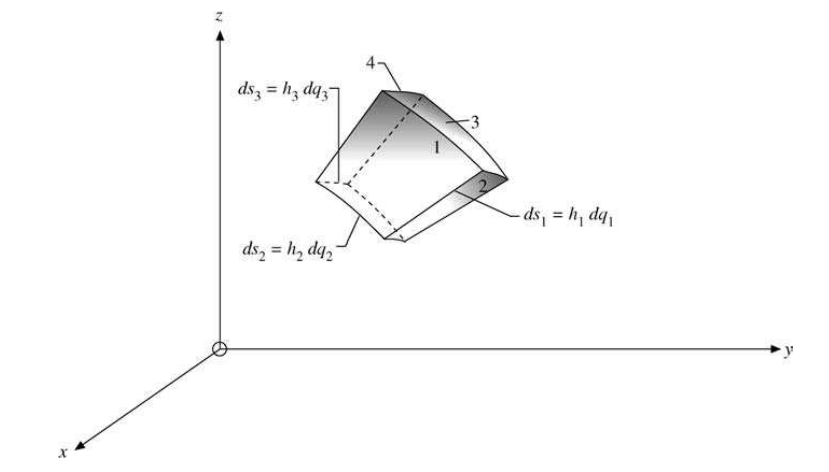
\includegraphics[scale=0.5]{Imagenes/ElementoVolumen_01.png}
    \caption{Elemento de volumen curvilíneo.}
\end{figure}
Nótese que las direcciones positivas se han elegido tal que $(\vu{q}_{1}, \vu{q}_{2}, \vu{q}_{3})$ o $(\vu{e}_{1},\vu{e}_{2}, \vu{e}_{3})$ forman un conjunto con orientación derecha: $\vu{q}_{1} \cp \vu{q}_{2} = \vu{q}_{3}$.
\par
La diferencia de área de las integrales para las dos caras $q_{1} = \text{constante}$ está dada por:
\begin{align}
\begin{aligned}
\left[ V_{1} \: h_{2} \: h_{3} + \pdv{q_{1}} (V_{1} \: h_{2} \: h_{3}) \: \dd{q_{1}} \right] \: \dd{q_{2}} \dd{q_{3}} -& V_{1} \: h_{2} \: h_{3} \: \dd{q_{2}} \dd{q_{3}} \\
=& \pdv{q} (V_{1} \: h_{2} \: h_{3}) \dd{q_{1}} \dd{q_{2}} \dd{q_{3}}
\end{aligned}
\label{eq:ecuacion_02_20}
\end{align}
Aquí  $v_{i} = \vb{V} \vdot \vu{q}_{i}$ es la proyección de $\vb{V}$ en la dirección  $\vu{q}_{i}$. Agregando los resultados que se obtienen de manera similar para las otras dos superficies, tenemos que:
\begin{align}
\begin{aligned}
\int \vb{V}(q_{1}, & q_{2}, q_{3}) \vdot \vu*{\sigma} =  \\
&= \left[ \pdv{q_{1}} (V_{1} \: h_{2} \: h_{3}) + \pdv{q_{2}} (V_{2} \: h_{3} \: h_{1}) +
\pdv{q_{3}} (V_{3} \: h_{1} \: h_{2}) \right] \: \dd{q_{1}} \dd{q_{2}} \dd{q_{3}}
\end{aligned}
\end{align}
Usando la ecuación (\ref{eq:ecuacion_02_19}), dividiendo por el diferencial de volumen, se tiene que
\begin{equation}
\vb{\nabla} \vdot \vb{V}(q_{1}, q_{2}, q_{3}) = \dfrac{1}{h_{1} \: h_{2} \: h_{3}} \; \left[ \pdv{q_{1}} (V_{1} \: h_{2} \: h_{3}) + \pdv{q_{2}} (V_{2} \: h_{3} \: h_{1}) + \pdv{q_{3}} (V_{3} \: h_{1} \: h_{2})   \right]
\label{eq:ecuacion_02_21}
\end{equation}
De las ecuaciones (\ref{eq:ecuacion_02_18}) y (\ref{eq:ecuacion_02_21}), obtenemos el operador Laplaciano, usando $\vb{V} = \nabla \psi(q_{1} \: q_{2}\:  q_{3})$. Lo que nos devuelve
\begin{align}
\begin{aligned}
\nabla \vdot \nabla \psi (q_{1}, q_{2}, q_{3}) &= \\
&= \dfrac{1}{h_{1} \: h_{2} \: h_{3}} \left[ \pdv{q_{1}} \left( \dfrac{h_{2} \: h_{3}}{h_{1}} \pdv{\psi}{q_{1}} \right) + \right. \\
&+ \left.  \pdv{q_{2}} \left( \dfrac{h_{3} \: h_{1}}{h_{2}} \pdv{ \psi}{q_{2}} \right) + \pdv{q_{3}} \left( \dfrac{h_{1} \: h_{2}}{h_{3}} \pdv{\psi}{q_{3}} \right) \right]  
\end{aligned}
\label{eq:ecuacion_02_22}
\end{align}
\subsection{Rotacional.}
Para desarrollar el rotacional $\nabla \cp \vb{V}$, usamos el teorema de Stokes, en conjunto con la divergencia, tomamos el límite cuando el elemento de superficie tiende a cero. Trabajando un componente a la vez, consideramos un elemento diferencial de superficie en la superficie curvilínea $q_{1} = \text{constante}$. De:
\begin{equation}
\int_{s} \nabla \cp \vb{V} \vdot \dd{\vb*{\sigma}} = \vu{q_{1}} \vdot \left( \nabla \cp \vb{V} \right) \; h_{2} \: h_{3} \dd{q_{2}} \dd{q_{3}}
\label{eq:ecuacion_02_23}
\end{equation}
el teorema de Stokes nos devuelve
\begin{equation}
\vu{q_{1}} \vdot \left( \nabla \cp \vb{V} \right) h_{2} \: h_{3} \: \dd{q_{2}} \dd{q_{3}} = \oint \vb{V} \cdot \dd{\vb{r}}
\label{eq:ecuacion_02_24}
\end{equation}
con la integral de línea que rodea la superficie $q_{1}=\text{constante}$. Siguiendo el bucle $(1, 2, 3, 4)$ de la figura
\begin{figure}[H]
    \centering
    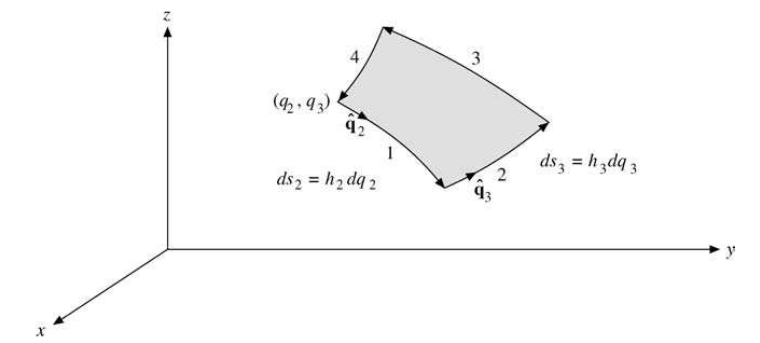
\includegraphics[scale=0.5]{Imagenes/ElementoCurvilineo_02.png}
    \caption{Elemento de superficie curvilíneo con $q_{1}=$ constante. }
\end{figure}
\begin{align}
\begin{aligned}
\oint \vb{V} (q_{1}, q_{2}, q_{3}) \vdot \dd{\vb*{r}} &= V_{2} \: h_{2} \dd{q_{2}} + \left[ V_{3} \: h_{3} + \pdv{q_{2}} (V_{3} \: h_{3}) \dd{q_{2}} \right] \: \dd{q_{3}} \\
&- \left[ V_{2} \: h_{2} + \pdv{q_{3}} (V_{2} \: h_{2}) \: \dd{q_{3}} \right] \: \dd{q_{2}} - V_{3} \: h_{3} \: \dd{q_{3}} \\
&= \left[ \pdv{q_{2}} (h_{3} \: V_{3}) - \pdv{q_{3}} (h_{2} \: V_{2}) \right] \: \dd{q_{2}} \dd{q_{3}}
\end{aligned}
\label{eq:ecuacion_02_25}
\end{align}
Se da un signo positivo cuando vamos en la dirección positiva de las partes 1 y 2, y un signo negativo en las partes 3 y 4, ya que vamos en dirección negativa. Los términos de orden mayor en la expansión de la serie de Maclaurin o de Taylor se omiten, ya que tienden a cero cuando el límite del elemento de superficie se hace muy pequeño ($\dd{q_{2}} \rightarrow 0, \dd{q_{3}} \rightarrow 0$.)
De la ecuación (\ref{eq:ecuacion_02_24}) tenemos
\begin{equation}
\nabla \cp \vb{V} \eval_{1} = \dfrac{1}{h_{2} \:h_{3}} \; \left[ \pdv{q_{2}} (h_{3} \: V_{3}) - \pdv{q_{3}} h_{2} \: V_{2} \right]
\label{eq:ecuacion_02_26}
\end{equation}
Las dos componentes que restan de $\nabla \cp \vb{V}$, se obtienen al realizar una permutación ciclíca de los índices. La mejor manera para escribir el rotacional, es una forma de determinante
\begin{equation}
\nabla \cp V = \dfrac{1}{h_{1} \: h_{2} \: h_{3}} \begin{vmatrix}
\vu{q}_{1} \: h_{1} & \vu{q}_{2} \: h_{2} & \vu{q}_{3} \: h_{3} \\[1em]
\displaystyle \pdv{q_{1}} & \displaystyle \pdv{q_{2}} & \displaystyle \pdv{q_{3}} \\[1em]
h_{1} \: V_{1} & h_{2} \: V_{2} & h_{3} \: V_{3}
\end{vmatrix}
\end{equation}
Recordemos que debido a la presencia de los operadores diferenciales, este determinante debe de expandrise de arriba hacia abajo. La ecuación en sí, no es idéntica a la forma del producto cruz de dos vectores, ya que $\nabla$ no es un vector común, es un operador vectorial.
\section{Sistema coordenado cartesiano}
Los factores de escala son:
\begin{align*}
\begin{aligned}
h_{1} &=& h_{x} = 1 \\
h_{2} &=& h_{y} = 1 \\
h_{3} &=& h_{z} = 1 \\
\end{aligned}
\end{align*}
Las siguientes expresiones corresponden para el gradiente, divergencia, laplaciano y rotacional:
\begin{align*}
\nabla \psi &= \vu{i} \pdv{\psi}{x} + \vu{j} \pdv{\psi}{y} + \vu{k} \pdv{\psi}{z} \\[1em]
\nabla \vdot \vb{V} &= \pdv{\psi}{x} + \pdv{\psi}{y} + \pdv{\psi}{z} \\[1em]
\nabla \vdot \nabla \psi &= \pdv[2]{\psi}{x} + \pdv[2]{\psi}{y} +  \pdv[2]{\psi}{z} \\[1em]
\nabla \cp \vb{V} &= \begin{vmatrix}
\vu{i} & \vu{j} & \vu{k} \\
\displaystyle \pdv{x} & \displaystyle \pdv{y} & \displaystyle \pdv{z} \\
V_{x} & V_{y} & V_{z}
\end{vmatrix}
\end{align*}
\section{Sistema coordenado cilíndrico ($\rho,\varphi,z$)}
En el sistema coordenado cilíndrico las tres coordenadas curvilíneas del sistema generalizado $(q_{1}, q_{2}, q_{3})$, se renombran por $(\rho, \varphi, z)$. Las superficies coordenadas:
\begin{enumerate}
\item Los cilindros circulares tienen al eje $z$ como eje común, tal que:
\[ \rho =  (x^{2} + y^{2})^{1/2} = \text{constante} \]
\item Los semiplanos a través del eje $z$
\[ \varphi = \tan^{-1} \left(\dfrac{y}{x} \right) = \text{constante} \]
\item Los planos paralelos al plano $x-y$, como en el sistema cartesiano:
\[ z = \text{constante} \]
\end{enumerate}
\begin{figure}[!h]
\centering
\tdplotsetmaincoords{70}{120}
\begin{tikzpicture}[tdplot_main_coords][scale=0.75]
\tikzstyle{every node}=[font=\small]
\draw[thick,-latex] (0,0,0) -- (6,0,0) node[anchor=north east]{$x$};
\draw[thick,-latex] (0,0,0) -- (0,6,0) node[anchor=north west]{$y$};
\draw[thick,-latex] (0,0,0) -- (0,0,6) node[anchor=south]{$z$};
\draw [thick](0,0,0) circle (3);
\draw [thick](0,0,4) circle (3);
\draw [thick](1.9,-2.35,0) -- (1.9,-2.35,4) node[midway, left]{$\rho=\rho_1$ superficie};
\draw [thick](-1.9,2.35,0) -- (-1.9,2.35,4);
\filldraw[fill=orange, nearly transparent] (-4,-4,4) -- (4,-4,4) --  (4,5,4) -- (-4,5,4) -- (-4,-4,4);
\filldraw[fill=blue, nearly transparent] (0,0,4) -- (5.2,6,4) --  (5.2,6,0) -- (0,0,0) -- (0,0,4);
\filldraw [color=blue](2,2.25,4) circle (0.075cm) ;
\draw (-4,5,4) node[anchor=south]{$z=z_1$ plano};
\draw (5.2,6,0) node[anchor=south west]{$\varphi=\varphi_1$ plano};
\node at (1.8,1,4)  { $\rho_{1}(\rho_{1},\varphi_{1},z_{1})$};
\draw[ultra thick,-latex](2,2.25,4) -- (3,3.45,4) node[anchor=north] {$\bm{\rho}_{0}$};
\draw[ultra thick,-latex](2,2.25,4) -- (1,2.5,4) node[anchor=north west] {$\bm{\varphi}_{0}$};
\draw[ultra thick,-latex](2,2.25,4) -- (2,2.25,4.75) node[anchor=north west] {$\mathbf{k}$};
\draw [thick,->](4,0,0) arc (0:45:4 and 4.5);
\draw (3.6,2,0) node[anchor=north] {$\varphi_1$};
\draw[ultra thick,-latex](0,0,0) -- (2,2.35,0);
\draw (1,1,0) node[anchor=north] {$\rho_1$};
\draw [ultra thick] (2,2.25,4)--(1.95,2.25,0);
\draw[ultra thick](0.1,0,4) -- (-0.1,0,4) node[anchor=south west] {$z_1$};
\end{tikzpicture}
\caption{Coordenadas cilíndricas circulares.}
\end{figure}
Los límites de $\rho, \varphi$ y $z$, son:
\[ 0 \leq \rho < \infty, \hspace{1cm} 0 \leq \varphi \leq 2 \pi, \hspace{1cm} -\infty < z < \infty \]
Podemos recuperar las relaciones de transformación:
\begin{align*}
\begin{aligned}
x &= \rho \cos \varphi \\
y &= \rho \sin \varphi \\
z &= z
\end{aligned}
\end{align*}
Considerando los elementos de longitud $\dd{s_{1}}$, revisamos que los factores de escala son:
\begin{align*}
\begin{aligned}
h_{1} &=& h_{\rho} = 1 \\
h_{2} &=& h_{\varphi} = \rho \\
h_{3} &=& h_{z} = 1
\end{aligned}
\end{align*}
\begin{figure}[H]
    \centering
    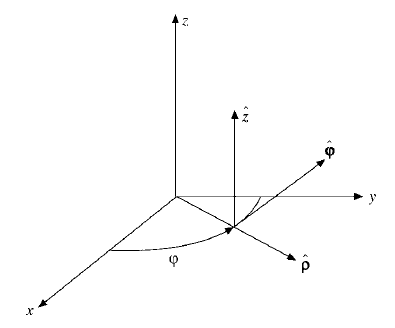
\includegraphics[scale=0.5]{Imagenes/CoordenadasCilindricas_Vector_Unitario.png}
    \caption{Vectores unitarios para el sistema coordenado cilíndrico circular.}
\end{figure}
Los vectores unitarios $(\vu{e}_{1},\vu{e}_{2},\vu{e}_{3})$ se renombran $(\vu*{\rho}_{0},\vu*{\varphi}_{0},\vu{z})$:
\begin{enumerate}
\item El vector unitario $\vu*{\rho}_{0}$ es normal a la superficie cilíndrica que apunta en la dirección del incremento del radio $\rho$.
\item El vector unitario $\vu*{\varphi}_{0}$ es tangencial a la superficie cilíndrica y además, perpendicular al semiplano $\varphi=\text{constante}$, y el vector apunta en la dirección del incremento del ángulo azimutal $\varphi$.
\item El vector $\vu{z}$, es el vector unitario que conocemos del sistema cartesiano.
\end{enumerate}
Estos vectores son mutuamente ortogonales
\[ \vu*{\rho} \vdot \vu*{\varphi} = \vu*{\varphi} \vdot \vu{z} = \vu{z} \vdot \vu*{\rho} = 0 \]
Un vector general $\vb{V}$ se expresa como
\[ \vb{V} =  \vu*{\rho} \: V_{\rho} + \vu*{\varphi} \: V_{\varphi} + \vb{z} \: V_{z} \]
Un elemento diferencial de desplazamiento $\dd{\vb{r}}$ se puede escribir como
\begin{align*}
\begin{aligned}
\dd{\vb{r}} &= \vu*{\rho}_{0} \dd{s_{\rho}} + \vu*{\varphi}_{0} \dd{s_{\varphi}} + \vu{z} \dd{z} \\
&= \vu*{\rho}_{0} \dd{\rho} + \vu*{\varphi}_{0} \: \rho \dd{\varphi} + \vu{z} \dd{z}
\end{aligned}
\end{align*}
Los operadores diferenciales, resultan ser:
\begin{align*}
\nabla \psi (\rho, \varphi, z) &= \vu*{\rho} \: \pdv{\psi}{\rho} + \vu*{\varphi} \: \dfrac{1}{\rho} \: \pdv{\varphi}{\varphi} + \vu{z} \: \pdv{\psi}{} \\[1em]
\vb{\nabla} \vdot \vb{V} &= \dfrac{1}{\rho} \pdv{\rho} (\rho \: V_{\rho}) + \dfrac{1}{\rho} \: \pdv{V_{\varphi}}{\varphi} + \pdv{V_{z}}{z} \\[1em]
\nabla^{2} \psi &= \dfrac{1}{\rho} \pdv{\rho} \left( \rho \: \pdv{\psi}{\rho} \right) + \dfrac{1}{\rho^{2}} \pdv[2]{\psi}{\varphi} + \pdv[2]{\psi}{z} \\[1em]
\vb{\nabla} \cp \vb{V} &= \dfrac{1}{\rho} 
\renewcommand\arraystretch{1.5} \begin{vmatrix}
\vu*{\rho} & \rho \: \vu*{\varphi} & \vu{z} \\
\displaystyle \pdv{\rho} & \displaystyle \pdv{\varphi} & \displaystyle \pdv{z} \\
V_{\rho} & \rho \: V_{\varphi} & V_{z}
\end{vmatrix}
\end{align*}
\textbf{Ejemplo: } Las ecuaciones de Navier Stokes de la hidrodinámica incluyen un término no lineal:
\[ \vb{\nabla} \cp [ \vb{v} \cp ( \vb{\nabla} \cp \vb{v})] \]
donde $\vb{v}$ es la velocidad del fluido. Para flujos a través de un tubo cilíndrico en la dirección $z$ se tiene que
\[ \vb{v} =  \vu{z} \: v (\rho) \]
Calculamos primeramente el rotacional
\begin{align*}
\vb{\nabla} \cp \vb{v} = \dfrac{1}{\rho} \left| 
\renewcommand\arraystretch{1.5} \begin{matrix}
\vu*{\rho} & \rho \: \vu*{\varphi} & \vu{z} \\
\displaystyle \pdv{\rho} & \displaystyle \pdv{\varphi} & \displaystyle \pdv{z} \\
0 & 0 & v(\rho)\end{matrix} \right| = - \vu*{\varphi} \: \pdv{v}{\rho}
\end{align*}
ahora calculamos el doble producto escalar (vector con vector)
\begin{align*}
\vb{v} \times (\bm{\nabla} \times \mathbf{v}) = \left| 
\renewcommand\arraystretch{1.5} \begin{matrix}
\vu*{\rho} & \vu*{\varphi} & \vu{z} \\
0 & 0 & v \\
0 & - \displaystyle \pdv{v}{\rho} & 0 \end{matrix} \right| = - \vu*{\rho} \: v(\rho) \: \pdv{v}{\rho}
\end{align*} 
finalmente, el triple producto escalar resulta ser
\begin{align*}
\vb{\nabla} \cp ( \vb{v} \cp (\vb{\nabla} \cp \vb{v})) = \dfrac{1}{\rho} \left| 
\renewcommand\arraystretch{1.5} \begin{matrix}
\vu*{\rho} & \rho \: \vu*{\varphi} & \vu{z} \\
\displaystyle \pdv{\rho} & \displaystyle \pdv{\varphi} & \displaystyle \pdv{z} \\
v \: \displaystyle \pdv{v}{\rho} & 0 & 0 \end{matrix} \right| = 0
\end{align*}
Para este caso en particular, los términos no lineales se anulan. 
\section{Coordenadas polares esféricas $(r,\theta, \varphi)$}
Renombrando las coordenadas $(q_{1}, q_{2}, q_{3})$ como $(r, \theta, \varphi)$, vemos que el sistema coordenado esférico es consistente con:
\begin{enumerate}
\item Tenemos esferas concéntricas en el origen:
\[ r = (x^{2} + y^{2} + z^{2})^{1/2} =  \text{constante} \]
\item Hay conos circulares concéntricos en el eje $z$-polar, con vértices en el origen:
\[ \theta = \arccos \dfrac{z}{(x^{2} + y^{2} + z^{2})^{1/2}} = \text{constante}\]
\item Tenemos que los semiplanos pasan a través del eje $z$-polar:
\[ \varphi = \arctan\left(\dfrac{y}{x} \right) =  \text{constante}\]
\end{enumerate}
% %\begin{center}
% %\begin{figure}
% %\begin{tikzpicture}
% %\draw [dashed] (0,0) arc (180:0:4 and 2) ;
% %\draw (0,0) arc (180:360:4 and 2) ;
% %\draw [dashed] (0,0.5) arc (180:0:3.95 and 2) ;
% %\draw (0,0.5) arc (180:360:3.95 and 2) ;
% %\draw (0,0) arc (180:0:4 and 4);
% %\end{tikzpicture}
% %\end{figure}
% %\end{center}
Dado que la elección del ángulo polar $\theta$, el ángulo azimutal $\varphi$, el eje $z$ merece un manejo especial. Las ecuaciones de transformación son:
\begin{align*}
\begin{aligned}
x &= r \sin \theta \cos \varphi \\
y &= r \sin \theta \sin \varphi \\
z &= r \cos \theta
\end{aligned}
\end{align*}
Midiendo $\theta$ en el cuadrante positivo del eje $z$ y $\varphi$ en el plano $x-y$ sobre el eje positivo $x$. Los rangos donde varían las coordenadas son $0 \leq r < \infty$, $0 \leq \theta \leq \pi$, y $ 0 \leq \varphi \leq 2 \pi$. Diferenciando las expresiones inversas, tenemos que 
\begin{align*}
\begin{aligned}
h_{1} &= h_{r} = 1 \\
h_{2} &= h_{\theta} = r \\
h_{3} &= h_{\varphi} = r \sin \theta 
\end{aligned}
\end{align*}
Lo que nos da un elemento de línea
\begin{align*}
\begin{aligned}
\dd{\vb{r}} = \vu{r} \dd{r} + \vu*{\theta} \: r \: \dd{\theta} + \vu*{\varphi} \: r \: \sin \theta \dd{\varphi}
\end{aligned}
\end{align*}
por tanto
\begin{align*}
\dd{s^{2}} = \dd{\vb{r}} \vdot \dd{\vb{r}} =  \dd{r^{2}} + r^{2} \dd{\theta^{2}} + r^{2} \: \sin^{2} \theta \: \dd{\varphi^{2}}
\end{align*}
En este sistema coordenado esférico, el elemento de área (para $r=\text{constante}$) es:
\begin{align*}
\dd{A} = \dd{\sigma_{\theta \varphi}} = r^{2} \: \sin \theta \dd{\theta} \dd{\varphi}
\end{align*}
que se muestra en la siguiente figura:
\begin{figure}[H]
    \centering
    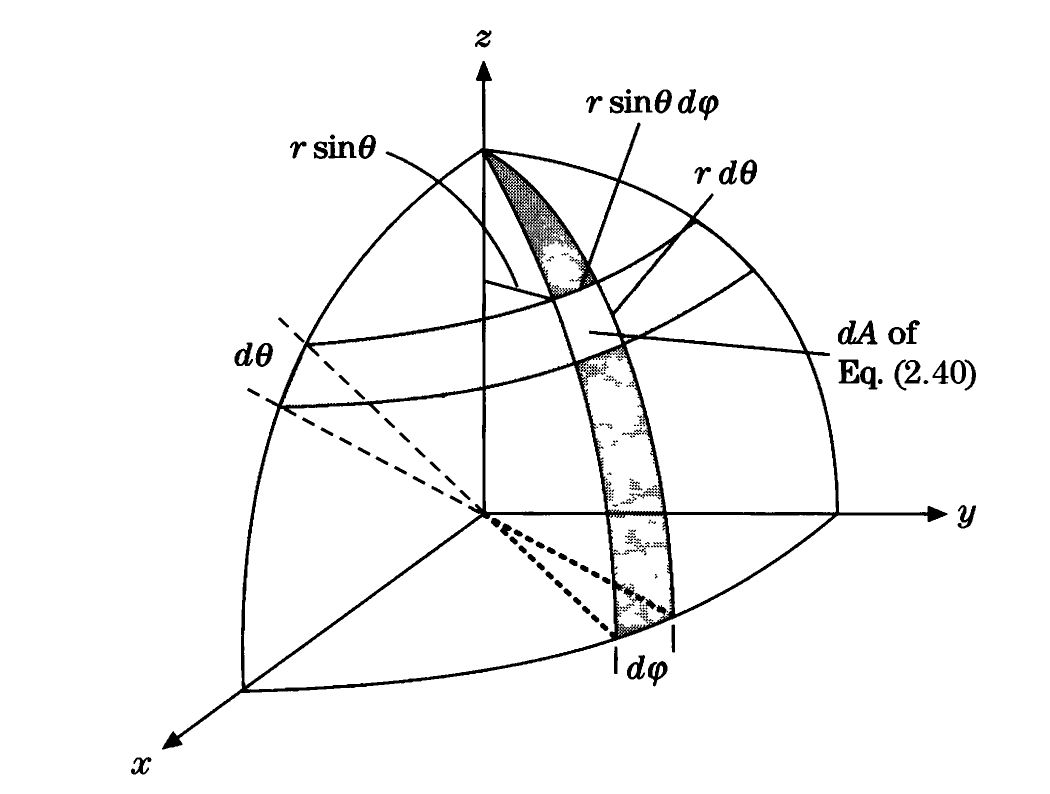
\includegraphics[scale=0.3]{Imagenes/Elemento_Area_Esferico.png}
    \caption{Elementos de área para un sistema coordenado esférico.}
\end{figure}
Integrando sobre la coordenada azimutal $\varphi$, se tiene que el elemento de área, genera un anillo de ancho $\dd{\theta}$
\[ \dd{A_{\theta}} = 2 \: \pi \: r^{2} \: \sin \theta \dd{\theta} \]
Esta expresión se presenta frecuentemente en problemas con coordenadas esféricas polares con simetría azimutal, tales como la dispersión de un haz no polarizado de partículas nucleares.
\par
Por definición de estereoradianes, un elemento de ángulo sólido $\dd{\Omega}$ está dado por:
\[ \dd{\Omega} = \dfrac{\dd{A}}{r^{2}} = \sin \theta \dd{\theta} \dd{\varphi} \]
Integrando sobre toda la superficie esférica, se obtiene
\[ \int \dd{\Omega} = 4 \: \pi \]
El elemento de volumen es:
\begin{align*}
\begin{aligned}
\dd{\tau} &= r^{2} \dd{r} \sin \theta \dd{\theta} \dd{\varphi} \\
&= r^{2} \: \dd{r} \dd{\Omega}
\end{aligned}
\end{align*}
Los vectores unitarios del sistema polar esféricos se muestran en la siguiente figura:
\begin{figure}[H]
    \centering
    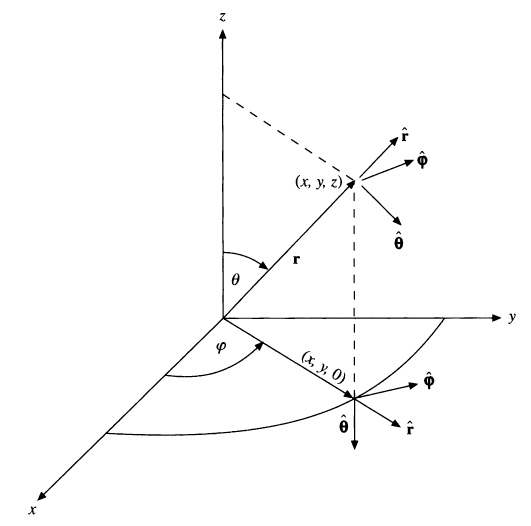
\includegraphics[scale=0.4]{Imagenes/CoordenadasEsfericasVectoresUnitarios.png}
    \caption{Vectores unitarios en coordenadas esféricas.}
\end{figure}
Se insiste en que los vectores unitarios $\vu{r}, \vu*{\theta}, \vu{\varphi}$ cambian de dirección conforme cambian los ángulos $\theta$ y $\varphi$. En términos de los vectores unitarios cartesianos $(\vu{i},\vu{j},\vu{k})$ cuya dirección es fija, tenemos que
\begin{align}
\begin{aligned}
\vu{r} &= \vu{x} \: \sin \theta \cos \varphi + \vu{y} \: \sin \theta \: \sin \varphi + \vu{z} \: \cos \theta \\
\vu*{\theta} &= \vu{x} \: \cos \theta \: \cos \varphi + \vu{y} \: \cos \theta \: \sin \varphi - \vu{z} \: \sin \theta = \pdv{\vu{r}}{\theta} \\
\vu*{\varphi} &= - \vu{x} \: \sin \varphi + \vu{y} \: \cos \varphi = \dfrac{1}{\sin \theta} \pdv{\vu{r}}{\varphi}
\end{aligned}
\end{align}
por lo que se tiene que
\begin{align*}
0 = \pdv{\vu{r}^{2}}{\theta} =  2 \: \vu{r} \vdot \pdv{\vu{r}}{\theta}, \hspace{2cm} 0 = \pdv{\vu{r}^{2}}{\varphi} =  2 \: \vu{r} \vdot \pdv{\vu{r}}{\varphi}
\end{align*}
Dadas la transformación inversa y un vector dado, se puede expresar de diferentes maneras, por ejemplo el vector de posición $\vu{r}$ puede escribirse como
\begin{align*}
\vb{r} &= \vu{r} \: r = \vu{r} \: (x^{2} + y^{2} + z^{2})^{1/2} \\
&= \vu{x} \: x + \vu{y} \: y + \vu{z} \: z  \\
&= \vu{x} \: r \: \sin \theta \: \cos \varphi + \vu{y} \: r \:  \sin \theta \: \sin \varphi + \vu{z} \: r \:  \cos \theta    
\end{align*}
De  acuerdo al problema a resolver, debemos de elegir la expresión más útil.
\par
Renombrando los vectores unitarios del sistema de coordenadas curvilineas $(\vu{q}_{1}, \vu{q}_{2}, \vu{q}_{3}) $ como $(\vu{r}, \vu*{\theta}, \vu*{\varphi})$, los operadores diferenciales para este sistema coordenado son:
\begin{align}
\nabla \psi &= \vu{r} \pdv{\psi}{r} + \vu*{\theta} \: \dfrac{1}{r} \: \pdv{\psi}{\theta} + \vu*{\varphi} \: \dfrac{1}{r \sin \theta} \: \pdv{\psi}{\varphi} \\[1em]
\vb{\nabla} \vdot \vb{V} &= \dfrac{1}{r^{2} \: \sin \theta} \left[ \sin \theta \: \pdv{r}(r^{2} \: V_{r}) + r \: \pdv{\theta} (\sin \theta \: V_{\theta}) + r \: \pdv{V_{\varphi}}{\varphi} \right] \\[1em]
\nabla \vdot \nabla \psi &= \dfrac{1}{r^{2} \: \sin \theta} \left[ \sin \theta \: \pdv{r} \left( r^{2} \: \pdv{\psi}{r} \right) + \pdv{\theta} \left( \sin \theta \: \pdv{\psi}{\theta} \right) + \dfrac{1}{\sin \theta} \: \pdv[2]{\psi}{\varphi} \right] \\[1em]
\vb{\nabla} \times \vb{V} &= \dfrac{1}{r^{2} \: \sin \theta}
\renewcommand\arraystretch{1.5} \begin{vmatrix}
\vu{r} & r \: \vu{\theta} & r \: \sin \theta \vu*{\varphi} \\
\displaystyle \pdv{r} & \displaystyle \pdv{\theta} & \displaystyle \pdv{\varphi} \\
V_{r} & r \: V_{\theta} & r \: \sin \theta \: V_{\varphi}
\end{vmatrix}
\end{align}
% \section{Construcción de sistemas coordenados.}
% Para construir un sistema de coordenadas en un espacio euclidiano basta contar con una familia de curvas planas, definida en forma tal que a cada valor de un parámetro le corresponda una curva. La teoría vista nos permite construir una familia de curvas ortogonales a la familia original. De este modo se obtiene un sistema de coordenadas curvilíneas ortogonales en el plano. Por rotación o adición del eje $z$ pueden generarse sistemas coordenados en 3D. Así, las coordenadas cilíndricas y esféricas pueden ser obtenidas de las coordenadas polares incluyendo el eje $z$ o rotando alrededor del eje $y$.
% \subsection*{Coordenadas parabólicas cilíndricas.}
% La ecuación de la familia de parábolas confocales, cuyo foco coincide con el origen de coordenadas tiene la forma:
% \begin{equation}
% y^{2} = 4 p (p + x)
% \label{eq:ecuacion_cpc_01_50}
% \end{equation}
% La cúspide de estas parábolas apunta a la izquierda. Para cada valor de $p: 0 \to \infty$, hay una parábola. El conjunto de parábolas con diferente valor de $p$ pero el mismo foco es \emph{confocal}. Si escribimos
% \[ f(x,y) = y^{2} - 4p(p+x) \]
% se tiene que
% \begin{equation}
% \nabla f = - 4 p \mathbf{\widehat{e}_{x}} + 2 y \mathbf{\widehat{e}_{y}}
% \label{eq:ecuacion_cpc_01_51}
% \end{equation}
% es un vector perpendicular a la curva (\ref{eq:ecuacion_cpc_01_50}), para un valor específico de $p$. Con el fin de que $\nabla f$ sea perpendicular a todas las parábolas debemos de eliminar $p$ de la ec. (\ref{eq:ecuacion_cpc_01_51}), usando la ec. (\ref{eq:ecuacion_cpc_01_50}). Se sigue que: $2p = -x + \sqrt{x^{2} + y^{2}}$ para $p \geq 0$, por lo que
% \[  \nabla f =  -2 \left( -x + \sqrt{x^{2} + y^{2}} \right) \mathbf{\widehat{e}_{x}} + 2 y \mathbf{\widehat{e}_{y}}  \]
% La ecuación de las curvas ortogonales a la familia de parábolas es $\nabla f \times d \mathbf{r} = 0$ de donde sigue con $d \mathbf{r} = \mathbf{\widehat{e}_{x}} dx + \mathbf{\widehat{e}_{y}} dy$:
% \[ y dx +  \left( - x + \sqrt{x^{2} + y^{2}} \right) dy = 0 \]
% si hacemos $y = vx$, tendremos
% \[ \dfrac{dv}{v} \left[ 1 - \dfrac{1}{\sqrt{1 + v^{2}}} \right] + \dfrac{dx}{x} = 0 \]
% de donde
% \begin{equation}
%  y^{2} = 4c (c -x)
%  \label{eq:ecuacion_cpc_01_52}
% \end{equation}
% Esta es otra familia de parábolas confocales cuya cúspide apunta a la derecha. Usaremos $c \geq 0$. Con las familias (\ref{eq:ecuacion_cpc_01_50}) y (\ref{eq:ecuacion_cpc_01_52}) definimos las coordenadas parabólicas.
% \\
% Para cada pareja $(p, c)$ hay un pareja de parábolas ortogonales que se cruzan en un punto al que llamaremos $(p, c)$, correspondiente a $(x, y)$.
% \\
% Por defnición las coordenadas parabólicas planas $(\eta, \xi)$ son:
% \[ 2p = \eta^{2} \hspace{1cm} 2c = \xi^{2} \]
% La regla de transformación entre coordenadas cartesianas y parábolcias planas, tiene entonces la forma:
% \[ x = \dfrac{\xi^{2} - \eta^{2}}{2} \hspace{1cm} y = \eta \xi \]
% Escogemos $\eta:0 \to \infty$. Con el fin de lograr que $y = \eta \xi$ pueda tomar valores negativos hemos de escoger $\xi = -\infty to \infty$.
% \\
% Definimos las coordenadas \textbf{parabólicas cilíndricas} adicionando la coordenada cartesiana $z$ a las coordenadas parabólicas planas $(\eta, \xi)$. En este caso:
% \begin{eqnarray*}
% \mathbf{r} &= x \mathbf{\widehat{i}} + y \mathbf{\widehat{j}} + \mathbf{\widehat{k}}  \nonumber \\
% &= \dfrac{\mathbf{\widehat{i}}}{2} \left( \xi^{2} - \eta^{2} \right) + \eta \xi \mathbf{\widehat{j}} + z \mathbf{\widehat{k}}
% \end{eqnarray*}
% Por lo que los factores de escala son
% \[ h_{\xi} = h_{\eta} = \sqrt{\xi^{2} + \eta^{2}}, h_{z} = 1  \]
% Si en vez de adicionar la coordenada $z$ realizamos una rotación de las coordenadas parabólicas planas alrededor del eje $x$ obtendremos, en vez de $y$, dos nuevos ejes $y$, y $z$ y una nueva coordenada $\varphi$, tal que: $y = \eta \xi \cos \varphi$ y $z= \eta \xi \sin \varphi$.
% \\
% Esta rotación da lugar a dos familias de paraboloides de revolución que originan un sistema de coordenadas parabólicas.
% \\
% En este caso, y después de reemplazar $x \to z$; $y \to x$; $z to y$ podemos escribir:
% \[ x = \eta \xi \cos \varphi, \hspace{0.5cm} y = \eta \xi \sin \varphi, \hspace{0.5cm} z = \dfrac{\xi^{2} -\eta^{2}}{2} \]
% con $0 \leq \xi < \infty$, $0 \leq \eta < \infty$, $0 \leq \varphi \leq 2 \pi$. Es fácil demostrar que
% \[ h_{\xi} = h_{\eta} = \sqrt{\xi^{2} + \eta^{2}}, h_{\varphi} = \eta \xi  \]
% Las superficies coordenadas de este sistema son: dos familias de paraboloides de revolución alrededor del eje $z$ correspondientes a $\xi = \mbox{ constante}$ y $\eta = \mbox{ constante}$, y planos meridianos $\varphi = \mbox{ constante}$.
% \\
% El siguiente paso es calcular en coordenadas parabólicas.
% \begin{enumerate}
% \item $\nabla \varphi$.
% \item $\nabla \cdot A$.
% \item $\nabla \times A$.
% \item $\nabla^{2} \varphi$.
% \end{enumerate}
% \subsection*{Coordenadas cilíndricas esféricas $(u, \theta, z)$}
% Están dadas por:
% \begin{eqnarray}
% \begin{aligned}
% x &= a \cosh u \cos \theta \\
% y &= a \sinh u \sin \theta \\
% z &= z
% \end{aligned}
% \end{eqnarray}
% donde $a$ es una constante.
% \subsection*{Coordenadas toroidales $(\xi,\chi,\varphi)$}
% Están definidas por las ecuaciones de transformación:
% \begin{eqnarray}
% \begin{aligned}
% x &=& \dfrac{a \sinh \xi \cos \varphi}{\cosh \xi - \cos \chi} \\
% y &=& \dfrac{a \sin  \xi \sin \varphi}{\cosh \xi - \cos \chi} \\
% z &=& \dfrac{a \sin \chi}{\cosh \xi - \cos \chi}
% \end{aligned}
% \end{eqnarray}
\end{document}
